\section{PHÂN TÍCH VÀ THIẾT KẾ HỆ THỐNG}

\subsection{Trình bày lượt đồ Use-case và đặc tả Use-case}

\subsubsection{Các cấp bậc quản lý}

\textTo{
\begin{itemize}
\item Nhân viên bán tour tiếp nhận yêu cầu đặt tour và phản hồi lại cho khách hàng qua email hoặc gọi điện thoại
\item Nhân viên chăm sóc khách hàng tham gia vào hệ thống tư vấn và giải đáp cho khách hàng
\item Nhân viên bán tour là người phụ trách tiếp nhận giao dịch, cập nhật chổ và hỗ trợ bộ phận CSKH
\item Nhân viên quản lý tour (tour nội địa và tour quốc tế) là bộ phận quản lí cập nhật danh sách tour lên hệ thống và hỗ trợ bộ phận CSKH giải đáp thắc mắc của khách hàng
\item Kế toán viên sử dụng hệ thống để thống kê dữ liệu về kinh doanh, xuất báo cáo và tính lương cho nhân viên
\item Admin quản lí toàn bộ hệ thống, là người có quyền hạn cao nhất thực hiện được các chức năng của nhân viên, ngoài ra còn thêm chức năng quản lý thông tin user (thêm, xóa, chỉnh sửa)
\end{itemize}}

\vspace{10cm}

\begin{figure}[ht]
    \centering
    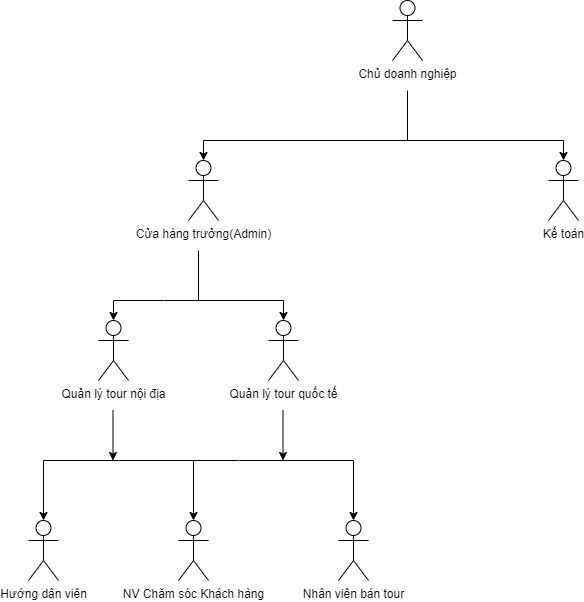
\includegraphics[width = 0.65\linewidth]{figures/Untitled Diagram.drawio (6).png}).png}
    \caption{Sơ đồ tổ chức cấp quản lý của  HAPPY TOUR.}
    \label{fig:example_1}
\end{figure}

\textTo{
\begin{itemize}
\item Khách hàng sử dụng tài khoản đăng nhập vào trang web (được phép tự đăng ký nếu chưa có) xem danh sách các tour, xem chi tiết một tour. Sau đó tiến thành đặt vé tour (nếu hài lòng) và thanh toán bằng thẻ ngân hàng hoặc thanh toán trực tiếp. 
\item Chat với bộ phận chăm sóc khách hàng nếu cần tư vấn và giải đáp thắc mắc.
\item Quản lý cập nhận thông tin cá nhân.
\end{itemize}

}

\begin{figure}[ht]
    \centering
    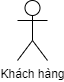
\includegraphics[width = 0.1\linewidth]{figures/Khách Hàng.png}
    \caption{Khách Hàng HAPPY TOUR.}
    \label{fig:example_1}
\end{figure}

\subsubsection{Các nhóm chức năng của hệ thống}

\begin{itemize}
\item Nhóm chức năng xem thông tin: Bao gồm xem tất cả thông tin khách hàng cho  phép, xem thông tin tour du lịch, chương trình khuyến mãi, ..., thông báo.
\item Nhóm chức năng quản lý: Quản lý nhân viên, quản lý thông tin tour du lịch, quản lý danh sách khách hàng tham gia tour, quản lý khuyến mãi, quản lý thông tin cá nhân khách hàng,...,quản lý tiền.
\item Nhóm chức năng tiếp nhận và xử lý: Kết nối liên lạc giữa khách hàng với các cấp quan lý, xử lý yêu cầu.
\end{itemize}

\subsubsection{Xác định các chức năng chính của hệ thống}

Tất cả các User phải đăng nhập mới được cấp quyền thực hiện các chức năng trong hệ thống ( ngoài trừ chức năng đăng ký của Khách Hàng)

\begin{figure}[ht]
    \centering
    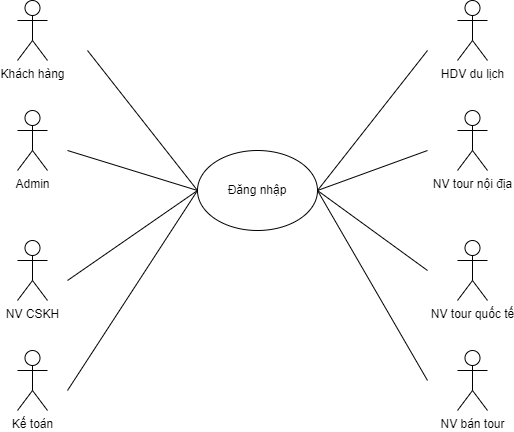
\includegraphics[width = 1.15\linewidth]{figures/Sub-UseCase-Đăng nhập.png}
    \caption{Chức năng đăng nhập.}
    \label{fig:example_1}
\end{figure}

\vspace{10cm}

\begin{enumerate}
\item Khách hàng


\begin{itemize}
\item Tạo tài khoản người dùng và đăng nhập vào Website và quản lí thông tin cá nhân.
\item Xem trang danh sách tour tổng quan, xem chi tiết tour, thanh toán qua ứng dụng thứ 3, theo dỗi hành trình di chuyển bằng app nội bộ được cung cấp khi đi tour.
\item Xem lại các tour đã đặt và đánh giá tour, hủy tour ( phải chờ phản hồi từ công ty)
\item Nhận thông báo về tour cũng như hóa đơn qua mail, nhận thông tin khuyến mãi.
\item Chat trực tuyến với bộ phận CSKH trên website
\end{itemize}

\begin{figure}[ht]
    \centering
    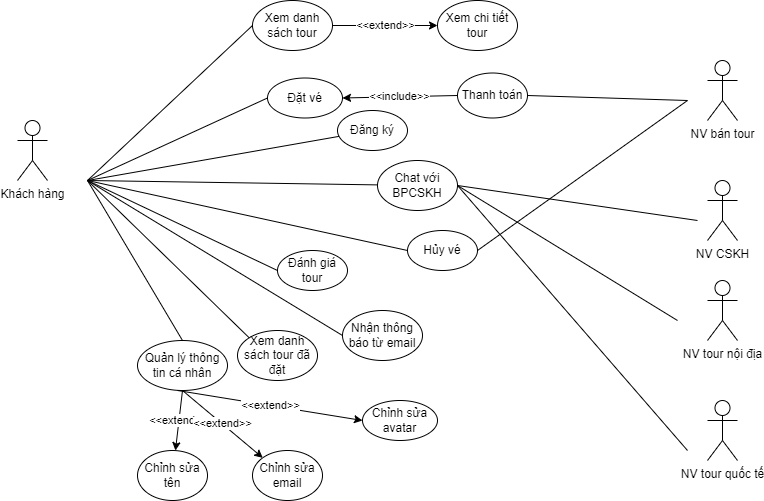
\includegraphics[width = 1.15\linewidth]{figures/Sub-UseCase-KhachHang.png}
    \caption{Chức năng của Khách Hàng.}
    \label{fig:example_1}
\end{figure}

\vspace{5cm}

\item Nhân viên phụ trách thông tin tour nội địa

\begin{itemize}
\item Được cung cấp tài khoản trang nội bộ để quản lí cập nhật (thêm, xóa, chỉnh sửa) thông tin tour du lịch nội địa ( bao gồm cả thông tin khách sạn và phương tiện di chuyển)
\item Được sử dụng chức năng trò chuyện trực tuyến trên website để hỗ trợ bộ phận CSKH.
\end{itemize}

\begin{figure}[ht]
    \centering
    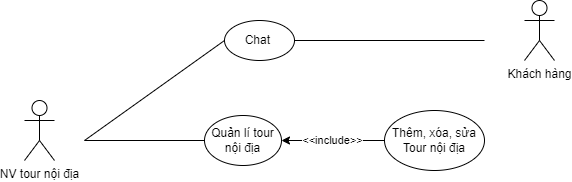
\includegraphics[width = 0.98\linewidth]{figures/Sub-UseCase-TourNoiDia.png}
    \caption{Sub UseCase Tour NoiDia.}
    \label{fig:example_1}
\end{figure}

\vspace{1cm}

\item Nhân viên phụ trách thông tin tour quốc tế

\begin{itemize}
\item Chức năng tương tự với nhân viên tour nội địa nhưng bổ sung thêm thông tin tiêm chủng và visa.
\end{itemize}

\begin{figure}[ht]
    \centering
    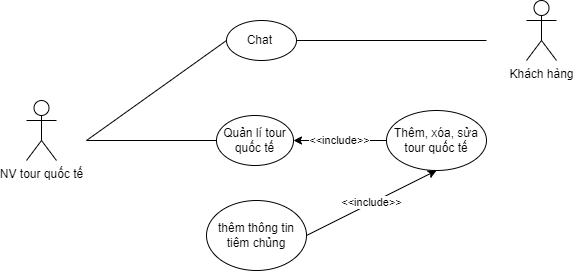
\includegraphics[width = 0.93\linewidth]{figures/Sub-UseCase-TourQuocTe.png}
    \caption{Sub UseCase Tour QuocTe.}
    \label{fig:example_1}
\end{figure}

\vspace{10cm}

\item Hướng dẫn viên du lịch (thuộc sở hữu của công ty)

\begin{itemize}
\item Xem những tour đã được phân công
\item Xem chi tiết thông tin tour bao gồm lịch trình, hành khách, phương tiện di chuyển, khách sạn.
\end{itemize}

\begin{figure}[ht]
    \centering
    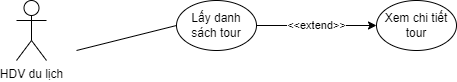
\includegraphics[width = 0.7\linewidth]{figures/Sub-UseCase-HDVdulich.png}
    \caption{Sub UseCase HDVdulich.}
    \label{fig:example_1}
\end{figure}

\item Nhân viên chăm sóc khách hàng

\begin{itemize}
\item Tư vấn và giải đáp các yêu cầu mà khách hàng gửi tin nhắn qua website.
\end{itemize}

\begin{figure}[ht]
    \centering
    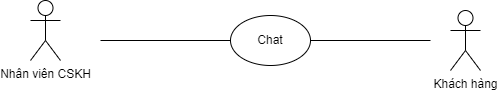
\includegraphics[width = 0.7\linewidth]{figures/Sub-UseCase-CSKH.png}
    \caption{Sub UseCase CSKH.}
    \label{fig:example_1}
\end{figure}

\item Kế toán

\begin{itemize}
\item Thống kê dữ liệu về tour và khách hàng và tài chính theo tuần, tháng, năm
\item Xuất báo cáo theo tuần, tháng, năm
\item Tính lương dựa theo số liệu điểm danh của phần mềm thứ 3 tích hợp dữ liệu sẳn vào hệ thống
\end{itemize}

\begin{figure}[ht]
    \centering
    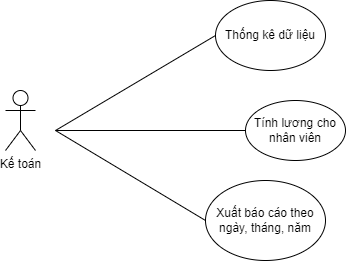
\includegraphics[width = 0.3\linewidth]{figures/Sub-UseCase-KeToan.png}
    \caption{Sub UseCase KeToan.}
    \label{fig:example_1}
\end{figure}

\item Nhiên viên bán tour

\begin{itemize}
\item Được cấp tài khoản nội bộ để xem danh sách tour và xử lý yêu cầu thanh toán, đồng thời phản hồi nếu có sự việc xảy ra.
\end{itemize}

\begin{figure}[ht]
    \centering
    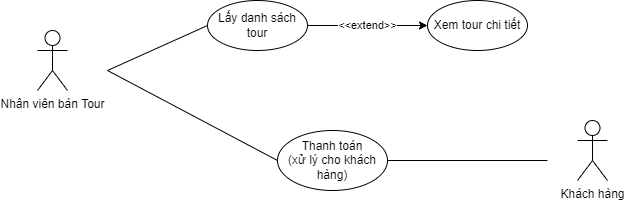
\includegraphics[width = 0.7\linewidth]{figures/Sub-UseCase-NVbanTour.png}
    \caption{Sub UseCase NVbanTour.}
    \label{fig:example_1}
\end{figure}

\vspace{5cm}

\item Cửa hàng trưởng - Admin

\begin{itemize}
\item Thực hiện được tất cả các chức năng của các nhân viên khác có toàn quyền trong hệ thống. 
\item Có thể phân bổ quyền hạn nhân viên.
\end{itemize}

\end{enumerate}

\begin{figure}[ht]
    \centering
    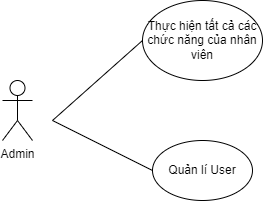
\includegraphics[width = 0.4\linewidth]{figures/Sub-UseCase-Admin.png}
    \caption{Sub-UseCase-Admin.}
    \label{fig:example_1}
\end{figure}

\vspace{10cm}

\begin{figure}[ht]
    \centering
    \includegraphics[width = 1.2\linewidth]{figures/Use Case.png}
    \caption{Sub-UseCase.}
    \label{fig:example_1}
\end{figure}

\vspace{10cm}




